\def\year{2015}
%File: formatting-instruction.tex
\documentclass[letterpaper]{article}
\usepackage{aaai}
\usepackage{times}
\usepackage{helvet}
\usepackage{courier}

\usepackage{graphicx}
\usepackage{subfigure}

\frenchspacing
\setlength{\pdfpagewidth}{8.5in}
\setlength{\pdfpageheight}{11in}
\pdfinfo{
/Title (Online Transfer Learning with Heterogeneous Source)
/Author (Author1, Author2, Author3)
/Keywords (Transfer Learning, Heterogeneous Transfer, Online Learning)
}
\setcounter{secnumdepth}{0}  
 \begin{document}
% The file aaai.sty is the style file for AAAI Press 
% proceedings, working notes, and technical reports.
%
\title{Online Transfer Learning with Heterogeneous Source}
\author{Author1\\ Address line\\
\And Author2 \\ Address line\\
\And Author3 \\ Address line\\
}
\maketitle
\begin{abstract}
\begin{quote}
AAAI creates proceedings, working notes, and technical reports directly from electronic source furnished by the authors. To ensure that all papers in the publication have a uniform appearance, authors must adhere to the following instructions. 
\end{quote}
\end{abstract}


\section{Introduction}

\section{Related Work}

\section{Online Heterogeneous Transfer}

\section{Experimental Results}

In this section, we empirically evaluate the performance of proposed online heterogeneous transfer learning algorithms and classic online Passive-Aggressive algorithms, which consists of a original version PA and its two variations PA-\uppercase\expandafter{\romannumeral1} and PA-\uppercase\expandafter{\romannumeral2}.
Encouraging results demonstrate that the proposed algorithms outperform baseline methods.

% dataset & task description
\subsection{Dataset}
Our experiments are conducted for image classification by leveraging information from text data.
We use NUS-WIDE dataset to generate learning tasks.
The NUS-WIDE dataset is extracted from Flickr.
It includes 269,648 images and the associated tags from Flickr, with a total number of 5,018 unique tags.
An image instance is represented by a feature vector based on SIFT descriptions, and a text instance is represented by a feature vector based on tags.
There are 81 ground-truth class labels in the dataset.
We randomly selected 10 classes (bird, boat, car, flower, food, rock, sun, toy, tree) and built $C_{10}^{2} = 45$ binary classification tasks.

We refer the images as data in the target domain, and the tags as the text data in the heterogeneous source domain.
Each binary classification task has 500 image instances in the target domain, 1,200 text instances in the heterogeneous source domain, and 1,500 co-occurred image-text pairs.
In order to obtain stable results, we draw 100 times of random permutation of the image instances in the target domain and evaluate the performance of learning algorithms based on average rate of mistakes.

\subsection{Baseline Methods}
We compare the proposed methods with Passive-Aggressive online learning algorithms.
PA algorithm proposed by Crammer et al. does not exploit knowledge from the source domain.
It deals with the traditional online learning problem in the target domain.
In addition, PA-\uppercase\expandafter{\romannumeral1} introduces a non-negative linear slack variable into PA, and PA-\uppercase\expandafter{\romannumeral2} introduces a quadratic slack variable.
Likewise, we have three versions of tow OHT algorithms (OHT$i$, OHT$i$-\uppercase\expandafter{\romannumeral1} and OHT$i$-\uppercase\expandafter{\romannumeral2}, where $i=\{1,2\}$) respectively based on PA algorithm and its variations.
We conduct three sets of experiments considering three versions separately.
Each set of experiments compares two OHT methods against a Passive-Aggressive algorithm.

For fair comparison and simplicity, we adopt Gaussian kernel function on all the algorithms and tasks.
The kernel parameter $\sigma = 8$ for the target domain.
The regularization parameter $C = 5$, $ \beta = \frac{\sqrt{T}}{\sqrt{T}+\sqrt{2\ln{4}}} $ for OHT2 algorithm.
In addition, we set the number of nearest neighbors to be considered $K = 100$.
Sensitivity of parameters will be examined in subsequent sections.

\subsection{Results and Discussion}
\begin{figure*}[!htb]
\centering
  \subfigure[PA-\uppercase\expandafter{\romannumeral2} vs OHT1-\uppercase\expandafter{\romannumeral2}]
  {
    \label{11}
    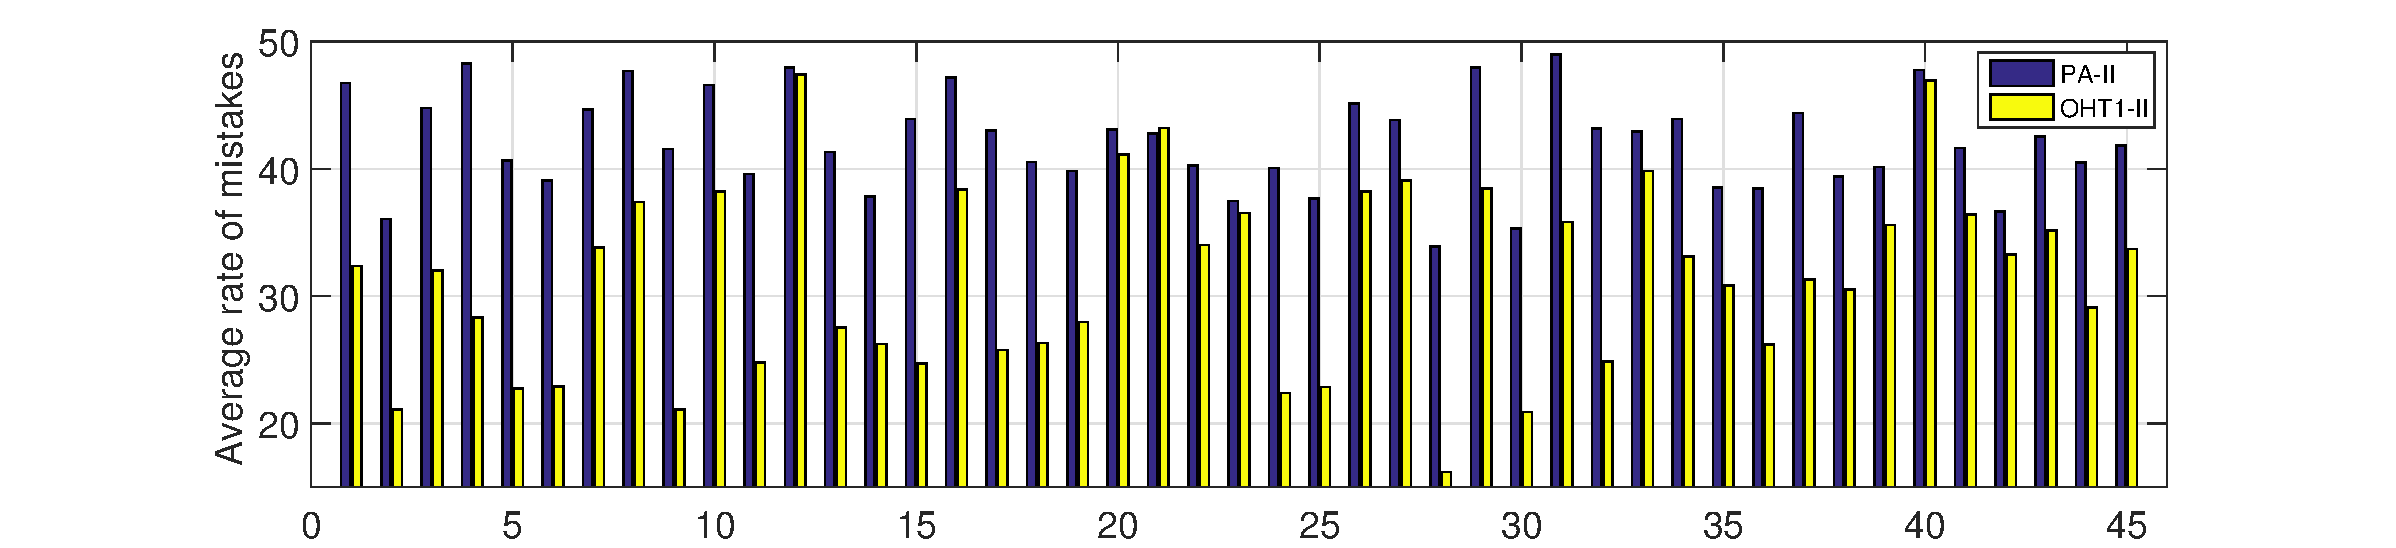
\includegraphics[width=18cm]{12_2.pdf}
  }
  \subfigure[PA-\uppercase\expandafter{\romannumeral2} vs OHT2-\uppercase\expandafter{\romannumeral2}]
  {
    \label{12}
    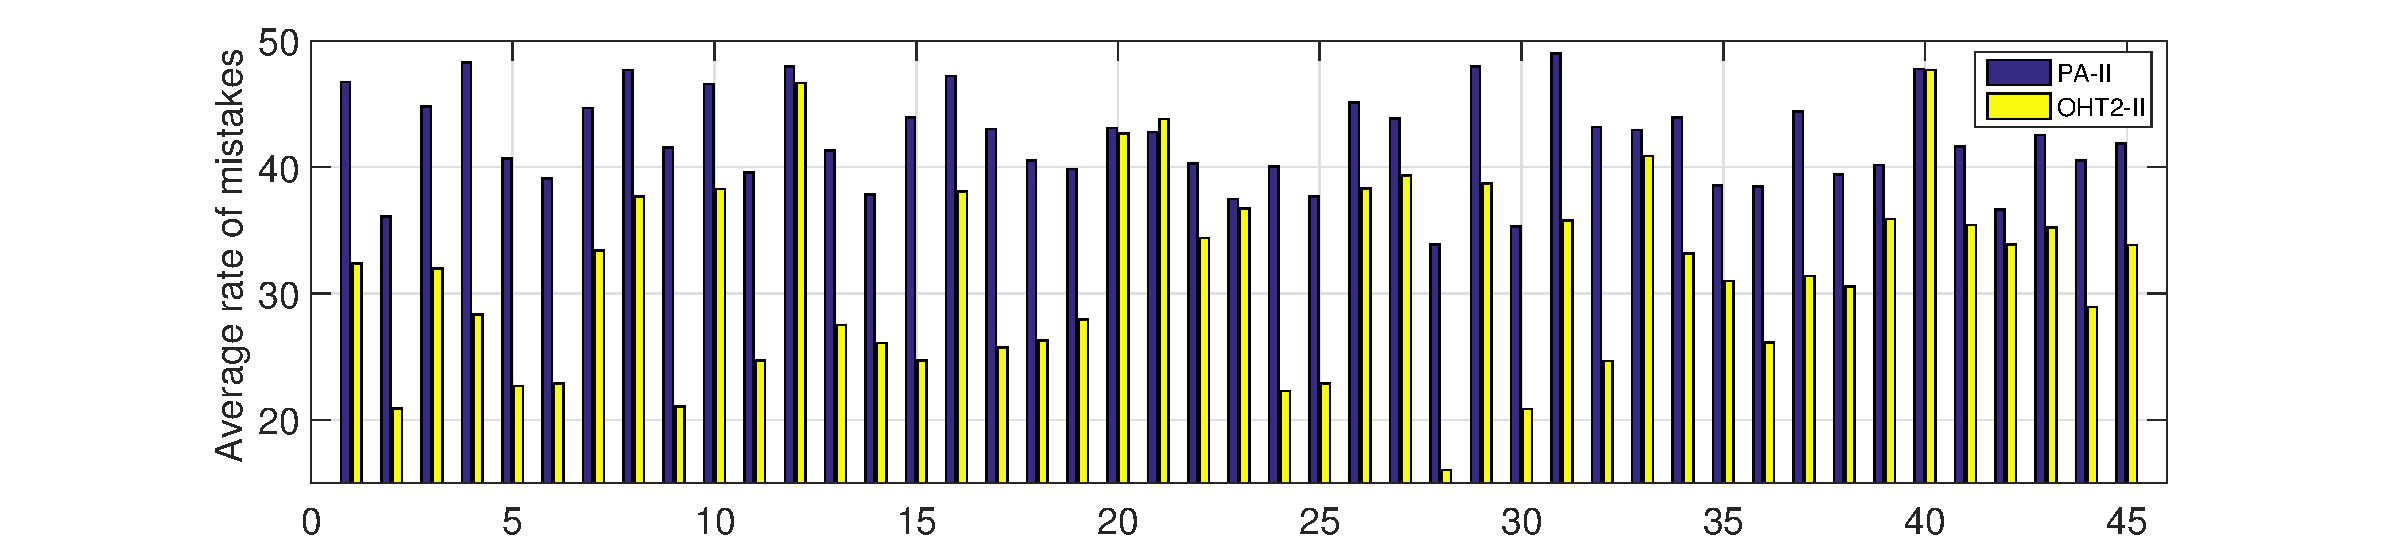
\includegraphics[width=18cm]{22_2.pdf}
  }
  \caption{Average rate of mistakes on all 45 tasks}
  \label{Average rate of mistakes on all 45 tasks}
\end{figure*}

Figure \ref{Average rate of mistakes on all 45 tasks} summarizes the mistake rates of all 45 binary classification tasks in the third set, which compares OHT1-\uppercase\expandafter{\romannumeral2}, OHT2-\uppercase\expandafter{\romannumeral2} and PA-\uppercase\expandafter{\romannumeral2}.
The x-axis of the figure refers to the 45 tasks.
We see that on most tasks, PA-\uppercase\expandafter{\romannumeral2} has the very high mistake rate, which prove the dificulty of image classification task without any auxiliary source information and the necessity of knowledge transfer.
The observation that our proposed OHT methods in general outperform Passive-Aggressive algorithm validates the effectivity of heterogeneous transfer learning.
Similar experimental results are observed in other two sets.
Because of the restricted space, we are not able to report them.
In order to facilitat the description, we denote PA-\uppercase\expandafter{\romannumeral2}, OHT1-\uppercase\expandafter{\romannumeral2} and OHT2-\uppercase\expandafter{\romannumeral2} by PA, OHT1 and OHT2 respectively in the following discussion.

\begin{figure*}[!htb]
\centering
  \subfigure[Task 2]
  {
    \label{task2}
    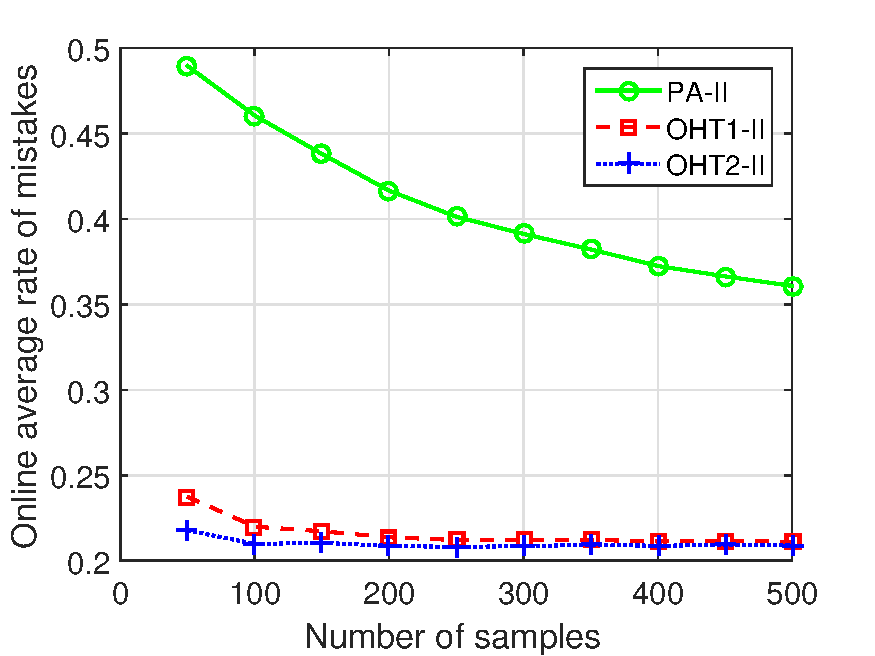
\includegraphics[width=5cm]{task2_2.pdf}
  }
  \subfigure[Task 14]
  {
    \label{task14}
    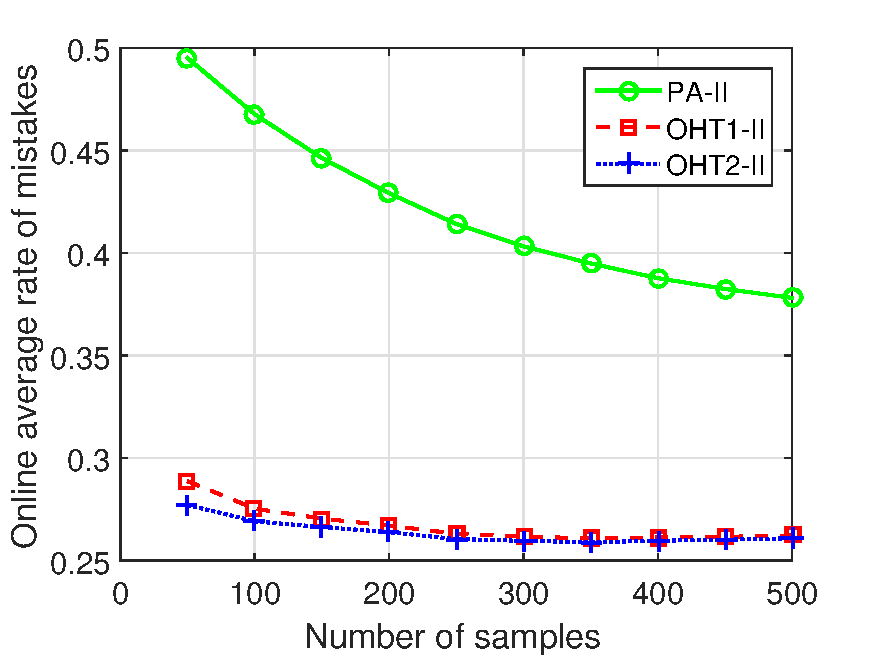
\includegraphics[width=5cm]{task14_2.pdf}
  }
  \subfigure[Task 36]
  {
    \label{task36}
    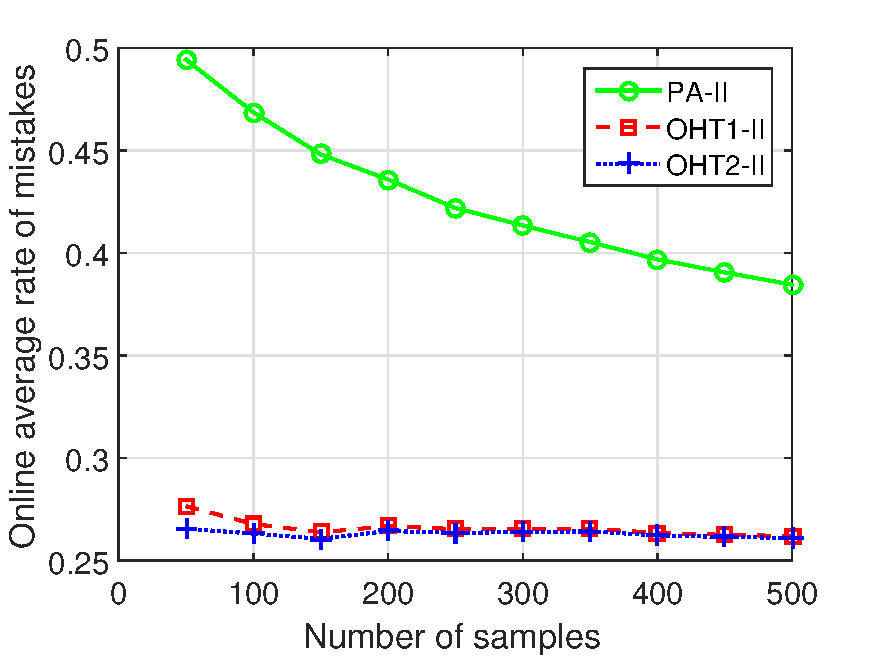
\includegraphics[width=5cm]{task36_2.pdf}
  }
  \\
  \subfigure[Task 7]
  {
    \label{task7}
    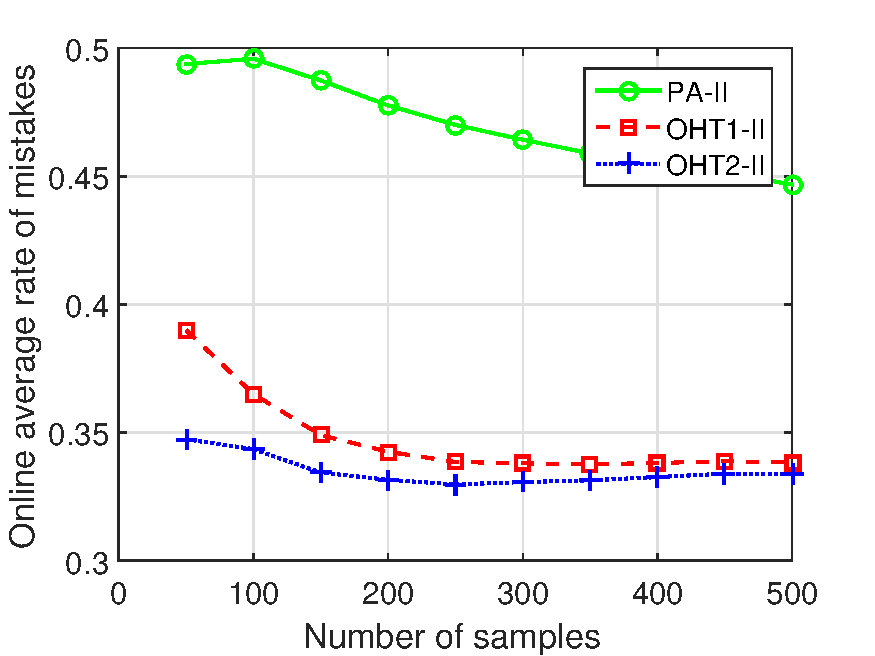
\includegraphics[width=5cm]{task7_2.pdf}
  }
  \subfigure[Task 16]
  {
    \label{task16}
    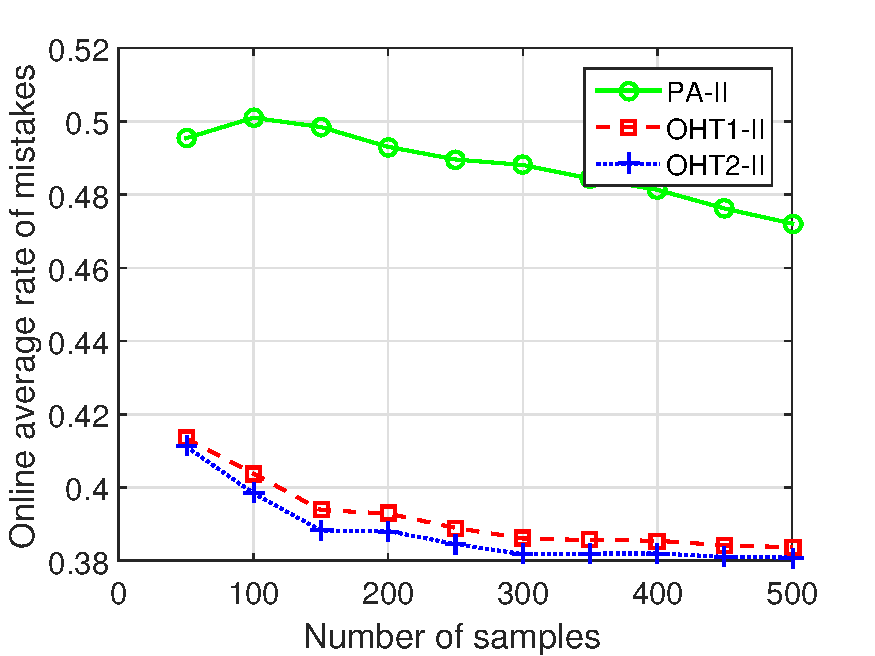
\includegraphics[width=5cm]{task16_2.pdf}
  }
  \subfigure[Task 33]
  {
    \label{task33}
    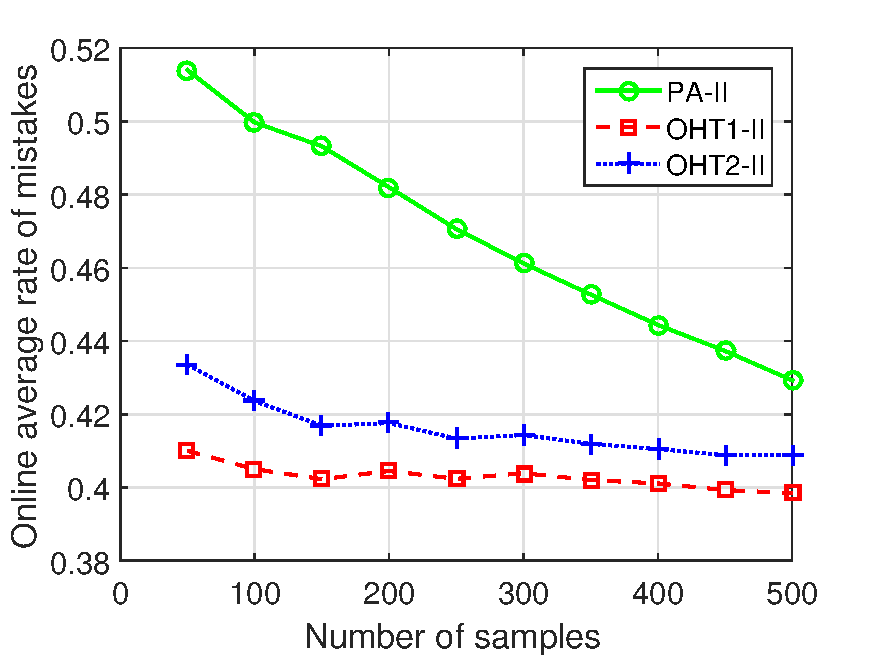
\includegraphics[width=5cm]{task33_2.pdf}
  }
  \caption{Online average rate of mistakes on example tasks}
  \label{Online average rate of mistakes on example tasks}
\end{figure*}

Figure \ref{Online average rate of mistakes on example tasks} illustrates the dynamic process of several representative online learning tasks, respectively.
We observe that OHT algorithms usually achieve better performance at the beginning stage.
On some tasks(e.g., 7, 16 and 33), the online mistake rates of all three algorithms decrease during the period, and OHT methods always obtain better performance than PA algorithm.
These observations verifies that the OHT algorithms indeed transfer useful knowledge from the heterogeneous source domain to the target domain. 

We also analyze the performance difference between PA and two OHT algorithms.
Statistical significance against PA was assessed by paired $t$-test at 0.01 level.
For each task, a win (or loss) is counted when OHT algorithm is significatly better (or worse) than PA algorithm over 100 trials.
Otherwise, a tie is recorded.
The win/tie/loss results is 44/0/1 for competition between OHT1 and PA, and 42/2/1 for competition between  OHT2 and PA.
This result validates that our OHT algorithms is statistically better than PA algorithm.

Besides, we utilize Cohen's $d$ value to measure the improvement of our algorithms.
Generally, $d>0.8$ indicates a large promotion, and $0.2<d<0.8$ indicates a middle promotion.
In our experiments, OHT1 algorithm achieves large improvement on 41 tasks and middle improvement on 3 tasks.
For OHT2 algorithms, the numbers are 40 and 3.
Combining the win/tie/loss results, we see that OHT1 is more stable than OHT2.


\subsection{Parameters and Running time}
% parameter sensitivity
\paragraph{Parameters}
Experiments in paper about online transfer learning illustrated that the performance of online transfer learning algorithms is generally insensitive to the parameter $C$ and $\beta$.
Consequently, we only investigate how different values of parameter $K$ affect the mistake rates of the algorithms.

\begin{figure}[!htb]
\centering
  \subfigure
  {
    \label{average_error}
    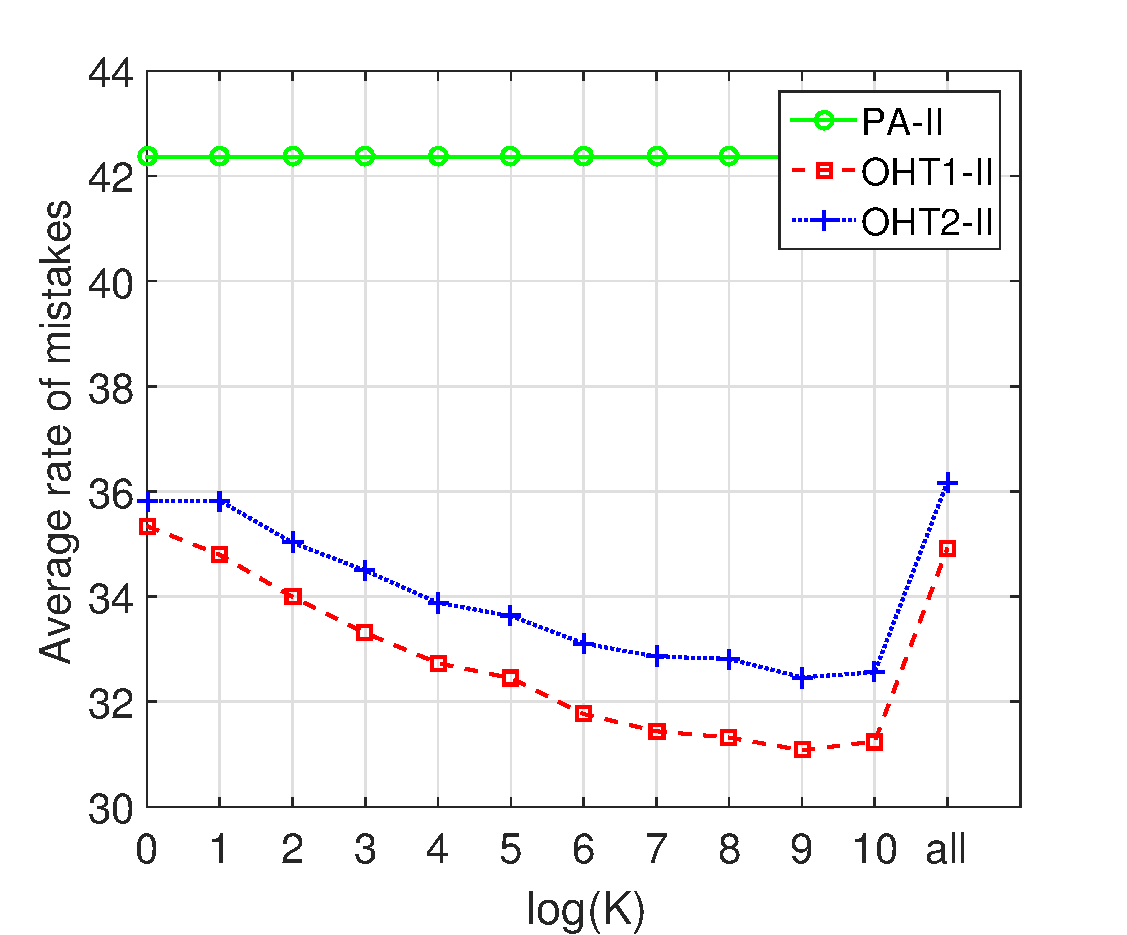
\includegraphics[width=3.9cm]{average_error.pdf}
  }
  \subfigure
  {
    \label{average_time}
    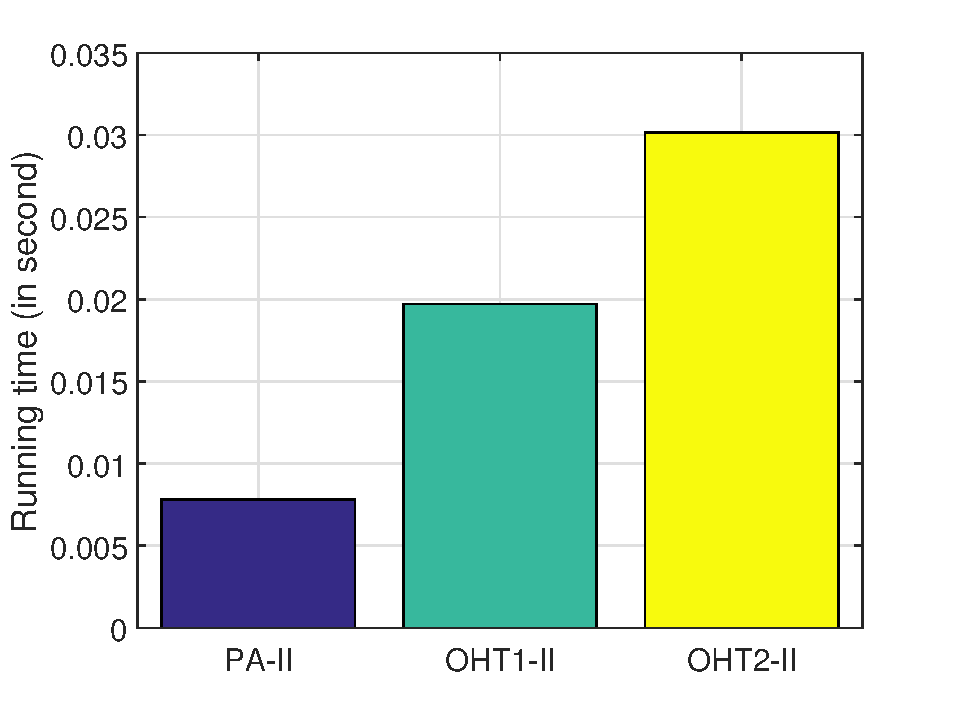
\includegraphics[width=3.9cm]{average_time.pdf}
  }
  \caption{(a) The average rate of mistakes under varying values of $K$. (b) The average running time of different algorithms}
  \label{average eok}
\end{figure}

Figure \ref{average eok} shows the average mistake rates with varied values of parameter $K$ over all 45 tasks.
PA algorithm, whose performance is not related to the parameter $K$, provide a baseline rate of mistakes.
We observe that the performance of the proposed methods consistently outperform PA algorithm, which indicates that nearest neighbors in heterogeneous source domain do provide valuable advice for the classification task.

% running time
\paragraph{Running time}
All of the algorithms were implemented in Matlab, and all experiments were run in a Linux machine with 3.2 GHz CPU and 3.8 GB memory.
Compared to PA algorithm without exploiting any information from the source domain, OHT algorithms are less efficient.
The main reason of more running time for OHT algorithms is probably the searching process for the nearest neighbors.
We can simply make use of all instances in the heterogeneous source domain to obtain generally comparable running time to PA, and at the same time, achieve better performance than PA.

\section{Conclusion}


\end{document}
\end{document}
